\documentclass{mprop}
\usepackage{graphicx}

% alternative font if you prefer
%\usepackage{times}

% for alternative page numbering use the following package
% and see documentation for commands
%\usepackage{fancyheadings}


% other potentially useful packages
%\uspackage{amssymb,amsmath}
\usepackage{url}
%\usepackage{fancyvrb}
%\usepackage[final]{pdfpages}

\begin{document}

%%%%%%%%%%%%%%%%%%%%%%%%%%%%%%%%%%%%%%%%%%%%%%%%%%%%%%%%%%%%%%%%%%%
\title{Is Technical Debt Real?}
\author{Ovidiu Popoviciu}
\date{18th December 2017}
\maketitle
%%%%%%%%%%%%%%%%%%%%%%%%%%%%%%%%%%%%%%%%%%%%%%%%%%%%%%%%%%%%%%%%%%%

%%%%%%%%%%%%%%%%%%%%%%%%%%%%%%%%%%%%%%%%%%%%%%%%%%%%%%%%%%%%%%%%%%%
\tableofcontents
\newpage
%%%%%%%%%%%%%%%%%%%%%%%%%%%%%%%%%%%%%%%%%%%%%%%%%%%%%%%%%%%%%%%%%%%

%%%%%%%%%%%%%%%%%%%%%%%%%%%%%%%%%%%%%%%%%%%%%%%%%%%%%%%%%%%%%%%%%%%
\section{Introduction}\label{intro}

\begin{itemize}
	\item What is technical debt?
	\item What are its applications?
	\item Why is it important?
\end{itemize}

Technical debt - definition \\
What impact does TD have on development?\\ 
How much work effort is wasted on new features on a codebase impacted with technical debt?\\
Why is it difficult to define such a measure? \\
If such a measurement is known, how could it be managed? \\
What are the advantages of quantifying technical debt interest in the form work effort? \\

Problem statement: Has the student analysed the problem, stated it clearly, and justified its importance?

%%%%%%%%%%%%%%%%%%%%%%%%%%%%%%%%%%%%%%%%%%%%%%%%%%%%%%%%%%%%%%%%%%%
\section{Background Survey}

\subsection{Study Design}

\begin{itemize}
	\item Technical debt definition
	\item Types of TD - focus on code debt
	\item Measurement of principal and interest
	\item Measurement of work effort and team productivity
	\item Management of TD
\end{itemize}

\subsection{Definition, Perspectives and Types}

% Ward Cunningham - WyCash Portfolio Management System
% TODO: expand the definition from the paper.
Technical debt is a metaphor termed by Ward Cunningham, in his famous report on the WyCash Portfolio Management System in 1993 \cite{Cunningham1993}.
In the report, Cunningham mentioned that "\textit{shipping first time code is like going into debt.}" and that as the system evolves new features would become more and more difficult to implement.
This phenomenon was due to feature-rich projects being shipped to customers early but poorly written with little or no consideration to quality and to future work.

\begin{figure}
	\centering
	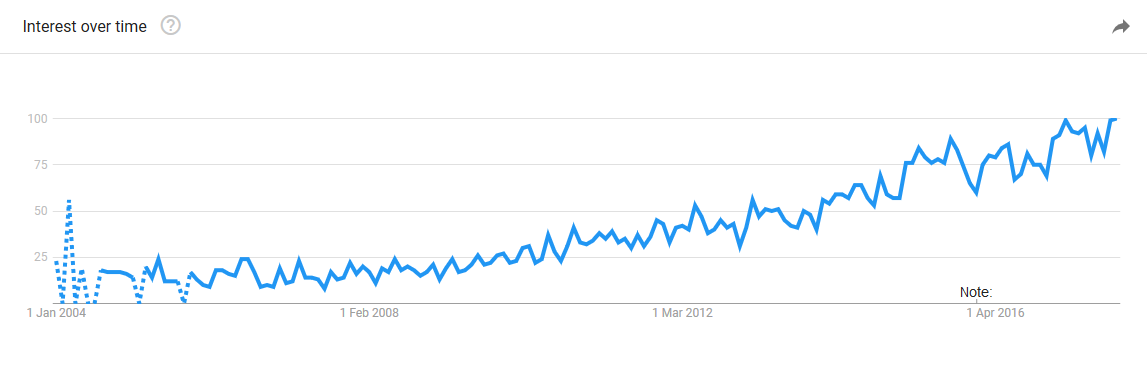
\includegraphics[width=\linewidth]{visualisations/TD_trend.png}
	\caption{Technical Debt Trend from 2004 to Present}
	\label{fig:td-trend}
\end{figure}

% MTD 2010
The metaphor was ignored for a long time, until the late 2000s, when more and more studies started to explore the phenomenon and possible management processes.
A figure of the popularity of Technical Debt from 2004 to present can be seen in Figure \ref{fig:td-trend}, information provided by Google Trends \cite{GoogleTrends}.
Thus, the first workshop on managing technical debt took place in 2010, where an initial research agenda was proposed for the future of software engineering field.
Since then, workshops have been held every year, which consisted seminars, presentations and brainstorming sessions on aspects such as
definition \cite{Kruchten2012} \cite{Theodoropoulos2011} \cite{Schmid2013},
identification \cite{Ernst2012},
measurement \cite{Letouzey2012} \cite{Curtis2012} \cite{Nugroho2011} \cite{Zazworka2011} \cite{Fontana2012} \cite{Bohnet2011},
management \cite{Guo2011} \cite{Zazworka2011Prioritise} \cite{Seaman2012} to
industry case studies \cite{Lim2012} \cite{Morgenthaler2012} \cite{Codabux2013} \cite{Holvitie2014} \cite{Klinger2011}.

% from metaphor to theory and practice
% TODO: add citation to industry case studies
The definition of technical debt relies heavily on the perspective of the viewer and her responsibility within the socio-technical environment.
Developers view technical debt as a list of software quality issues and correlate it with lack of time to implement features "\textit{properly}" \cite{Codabux2013}.
Product managers and stakeholders view at it as a strategy, a way to defer quality work for fast work in order to satisfy certain business requirements, such as Time to Market (TTM).
In practice, these two perspectives are widely different, with developers prioritising "invisible" code perfection whilst management focusing on rapid development of "visible", selling point features.
Kurchten et al. \cite{Kruchten2012} defined technical debt as technological gaps between development teams and management, where a gap is the evolution of a context specific to a decision taken in the past.
These gaps might have been decisions that seemed correct when the decision was taken however, with the passing of time, the initial decision incurred debt within the project.
For example, there is no tool that predicts what frameworks and languages will exist in the future or how to implement features by considering future unknown requirements.
As a consequence, the authors state that technical debt is not the collection of code quality violations within the results of static code analyzers but, a phenomenon which is heavily reliant on present and future project evolution.


% from a stakeholder's perspective
However, most strategic decisions on the future evolution of the project come from management.
Unfortunately, stakeholders might not have knowledge of the metaphor of technical debt, its current measurement and whether it impacts costs of development.
Their main focus of increasing business value through the addition of visual features, rather than looking for investment in the quality of the software being produced.
As a result, new features are prioritised and pressured on being delivered as early and as quickly as possible.
These types of issues affect the \textbf{extrinsic quality} of software and are "visible".
For example, an extrinsic quality characteristic is usability.
Deferring user experience work and ignoring user interface bugs might force users of the system to find "ways around" certain tasks.
The result is negative impact in user productivity and the general usefulness of the product.
Extrinsic characteristics are important to the business as they are considered "sell points" of the product.
On the other hand, \textbf{intrinsic quality} characteristics of software are the low-level issues such as code smells, best-practices violations that might slow down development of new features unless refactoring processes are applied.
Theodoropoulos et al. \cite{Theodoropoulos2011} considered that intrinsic and extrinsic software quality characteristics are interdependent and deferring quality maitainence in one area may affect other areas of quality.
For example, improper data validation in the business logic layer of the system, may impact downstream components, such as user interface, and produce bugs within the system.


% on the limits of td metaphor
% TODO: define principal and interest
Although the use of finance terms may simplify technical characteristics of software quality in the dialogue between development teams and stakeholders, the analogy breaks down as studied by Schimd et al. \cite{Schmid2013}.
In their study, the authors had identified shortcomings in the financial metaphor established by Ward Cunningham \cite{Cunningham1993} and found points where it breaks down.
In the financial domain, debt is a well known arrangement between two parties where one party borrowes a fixed amount of money from the other party \cite{debt-investopedia}.
The most well known types of debt are loans, where the terms of the arrangement dictate that the amount of money borrowed must be paid back in full after a fixed period of time, along with fixed interest payments paid annually.

Schmid et al. \cite{Schmid2013} has identified three major points where the analogy breaks down:
\begin{itemize}
	\item \textit{Unit of measurement}. In finance there is a clear unit of monetary measurement through the use of international currencies.
	      In contrast, technical debt does have a standard unit of measurement defined.
	      There are many tools (TODO: add citation of paper tools here) that provide a single, quantified and aggregated measure of the amount of time it takes for software quality issues to be resolved.
	      Additionally, very few of these tools quantify the consequences of neglecting refactoring and the improvement in quality characteristics.
	      The issue of measurement puts a dent into the shared vocabulary between development and stakeholders as mentioned by a number of software practioners from industry case studies (TODO: add industry case study citation here).
	\item \textit{Fixed time period}. On the one hand, debt arrangements have a fixed \textit{maturity date}, where the debt must be paid back.
	      On the other hand, software quality issues do not a have a time limit and may be kept in the product until they are resolved.
	      Fixing these items relate to paying back the "loan" taken on their creation.
	      Such issues may never be paid back if not needed to, resulting in an increased cost-value ratio.
	\item \textit{Fixed interest}. A loan arrangement additionally consists of fixed interest payments measured as a percetange of the loan value, paid on an annual or bi-annual basis.
	      The interest compensates for the risk taken by the lender and encourages the loanee to pay back quickly as possible in order to avoid paying back too much interest.
	      In reality, there is no such thing as fixed interest dependant on a single factor in technical debt.
	      Interest is difficult to quantify as a matter of principal, and the amount of interest paid after a period of time depends on future work.
\end{itemize}
Under these circumstances, what is considered "good structure" or "clean code" is also heavily influenced to future development since future decisions influence cost impact.
As a consequence, no system is \textit{debt free} and thus fixing every code violation would be an act of gold plating.
Additionally, what is the value of paying back this debt if the product is competitive and the customers are happy \cite{Lim2012}?

% martin fowler - td quadrants
In Martin Fowler's famous article \cite{TDMartin}, he described this type of future debt as \textbf{inadeverted-prudent} debt.
Over time, a project that was "clean" may find that after a period of time that the initial approach taken might not have been the best.
He considered that developers learn on the job to perfect their craft as time passes.
The four quadrants refer to the types of technical debt that one might encounter in a software project given the approach taken by the development team.
It was one of the four quandrants he defined, as shown in Figure \ref{fig:td-quandrants}.

\begin{figure}
	\centering
	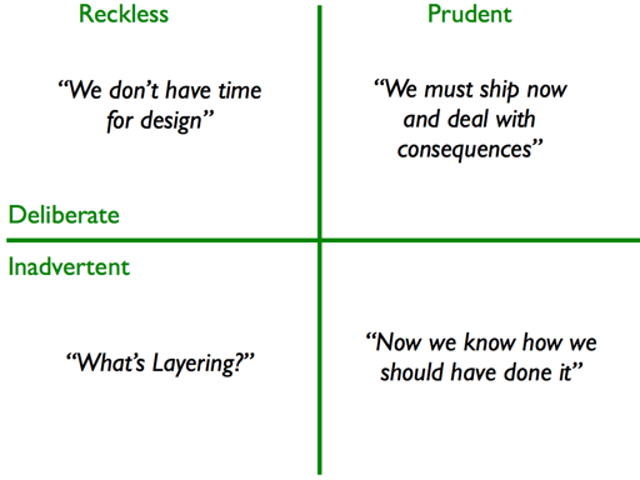
\includegraphics[width=0.5\linewidth]{visualisations/TD_quadrants.png}
	\caption{Martin Fowler's Technical Debt Quadrants}
	\label{fig:td-quandrants}
\end{figure}


% unhedged call option
An alternative metaphor of technical debt \cite{UnhedgedCallOption}, described bad code using finance terms in a similar fashion, but through a different financial intrument called a call option.
\textit{An option is a financial derivative that represents a contract sold by one party (the option writer) to another party (the option holder). The contract offers the buyer the right, but not the obligation, to buy (call) or sell (put) a security or other financial asset at an agreed-upon price (the strike price) during a certain period of time or on a specific date (exercise date).} \cite{option-investopedia}.
A call option gives the right to buy while a put option gives the option holder the right to sell.
In software engineering, if a feature is hacked up quickly using bad code and never touched again, then the project had reaped the rewards.
The option "was not called".
However, if a new feature were required that would be influenced by the quick and dirty work implemented earlier, then the requirement would be more expensive to fulfill.
In this case, the option "has been called".


% conclusion
Defining software quality issues as a financial metaphor helps bridge vocabulary shortcomings between developers and stakeholders.
It helps management understand current software development risks and encourages ways for managing these risks as they are created.
TODO: make sure to write down the exact definition
As Cunningham \cite{Cunningham1993} had written, technical debt may be used as a strategy in order to meet business expectations however, if not repaid promptly it could bring entire corporations to a standstill.

% types of TD
Initially, technical debt has solely focused on the internal quality issues of systems developed.
Such issues could be code smells, code violations and duplicate or complex code.
However, multiple types of debt have been "discovered" spanning the entire socio-technical environment.

% TODO: maybe add a description for all types of debt
% but only focus on code debt
A mapping study, conducted by Li et al. \cite{Li2015}, have analysed 94 papers, overall dating 1992-2013, and have found 10 types of technical debt being studied:
requirements debt,
architectural debt,
design debt,
code debt,
test debt,
build debt,
documentation debt,
infrastructure debt,
versioning debt
and defect debt.

The most prominent type of debt studied was code debt, followed by test, architectural, design and documentation debt.

% architecture debt is the worst - industrial case study
Developers of an industrial case study considered that architectural debt is the most difficult to adress, due to complexity and change impact on project \cite{Codabux2013}. 
Major architectural decisions are not taken in a vaccuum and thus requires group meetings with other developers, software architects and product managers.
The time to reach a consensus on how to approach such changes improve the cost of managing architectural debt.

% techical debt is "technical"
A few of the authors have considered that the metaphor of technical debt should only apply to the low-level, internal quality characteristics such as code, test, architectural debt rather than process gaps such as inadequate quality assurance \cite{Theodoropoulos2011} \cite{Nugroho2011}.
Thus the word "technical".
However, process gaps may negatively affect projects and incurr technical debt as a result.

%%%%%%%%%%%%%%%%%%%%%%%%%%%%%%%%%%%%%%%%%%%%%%%%%%%%%%%%%%%%%%%%%%%
\subsection{Identification and Measurement}

There are two methods for identifying technical debt within project source code:
manually found by developers during the design or implementation stages of a new feature or
automatically identified by a code quality tool that runs either in the integrated development environment of the developer or a project-level continous code quality tool.

There a number of authors who have studied the identification of technical debt and its measurement through the use of static analysis tools.
They scan the source code and find various code violations, such as code smells, code duplication, cyclomatic complexity, test coverage issues, etc.
Moreover, they can provide detailed quality reports, links to source code, custom violations and quality thresholds.

Fontana et al. \cite{Fontana2011} had compiled an initial report on code smell detection tools and their experience on the analysis of multiple versions of an object-oriented Java project.


\subsubsection{The SQALE Method for Measuring Technical Debt} \cite{Letouzey2012}
The goal of this paper was to propose a standardized, language-agnostic framework for assessing the quality of source code by deriving measures for important code characteristics and calculating technical debt.
The framework proposed consisted of four concepts:
\begin{itemize}
	\item Quality Model - defines internal properties of code through a structured three-layer hierarchy (characteristic, sub-characteristic and requirement).
	\item Analysis Model - measurement of the distance between the current state of the application and the \"optimized\" state, the quality target.
	\item Indices - each characteristic of the Quality Model defines a remediation index (cost to repair the non-compliances) defined in time, work or capital units.
	\item Indicators - provide a visual representation of technical debt either through ratings (ratios between TD and development cost) or SQALE Pyramids (distribution of TD over all the characteristics).
\end{itemize}

Each organization must manage technical debt as early as possible in a project with indicators and dashboards for code quality available for each build within the continous integration pipeline.
Quality model must be calibrated according to the requirements and policies of the organization implementing the framework. For example, to approve/decline rules that are considered debt and what principal costs are for each type of code violation.
One limitation is that the framework does not take into consideration other types of technical debt such as requirements debt, operational debt.
There is no standardized definition of right code, organizations have to define their own \"right\" code rules.

\subsubsection{Estimating the Size, Cost and Types of Technical Debt} \cite{Curtis2012}
Summarized the results of a study on a huge database (365M LOC) of software projects across 10 industries.
The study was language agnostic and provided a formula for estimating the principal of TD items.
Made use of CAST's Application Intelligence platform to statically analyse source code, using 1200 rules for good practices.
The steps taken were as follows: parsing, identify violations, aggregate results and sum up into a quality characteristics, or \textit{health factors}.
Scores from each health factor were aggregated on a scale of 1 (high risk) to 4 (low risk).
The principal was estimated by a formula with three parameters: number of problems, time required for each fix and the cost of fixing the issue.
The authors concluded that estimating the interest incurred by a TD item was difficult since might be multiple hidden factors which influenced the results.
The term works well with the phenomenon since stakeholders think of software quality in terms of business. \\
There are trade-offs of TD management from stakeholder's perspective.
For example, fixing TD items within the Robustness characteristic may lead to fewer operational failures and higher availability of the system.

\subsubsection{An Empirical Model of Technical Debt and Interest}  \cite{Nugroho2011}
The goal was to formally define technical debt and interest to provide insights on the Return On Investment (ROI) of IT executives.
Specifically, it tried to answer the following questions from a financial perspective: How large is TD? How much interest are paying? What are the consequences of holding on to debt?
The authors had completed an empirical analysis of 44 projects within the Software Improvement Group (SIG) using TUViT software quality assessment method for collecting relevant metrics: lines of code, code duplications, etc.
The had also defined technical debt as being the changes needed to bring a system from its current quality state to the "ideal" quality. This can be quantified as the repair effort (RE) and can be calculated as follows:
RE = Rework Fraction (LOC need to be changed) * Rebuild Value (estimate in man-months of rebuilding with a particular technology) * Refactoring Adjustment (advanced tooling helping the team be more productive.)\\
The interest was also derived from the extra cost spent on maintainance per month and per year, modelled against the quality factor (the current state of quality within the system).
Maintainance was considered a different activity by the authors since the tasks involved in maintaining a system involve a change that is immediately visible from the outside.
However, technical debt repair was not considered a maintainance activity.
A few limitations of this approach were the level of precision rating of a system (quality ratings are on a scale of 1-5) which leads to less accurate estimations on important financial numbers such as ROI.
Refactoring adjustment variable is subjective as it requires expert input when considering development productivity.

\subsubsection{Investigating the Impact of Design Debt on Software Quality} \cite{Zazworka2011}
To investigate the impact God classes have on development and whether they are points of major changes and defects when compared to other parts of the system. Additionally, to study whether there is a linear relationship between class size, change and defect likelihoods and how the results are influenced by data normalizations
The authors ran an analysis on two medium-sized projects from a small development company. The analysis consisted of statically analysing the source code stored in version control and the project issues from the project management system.
It looked at two major variables:
\begin{itemize}
\item Change likelihood = how likely code within and outside God classes changes accross revisions.
\item Defect likelihood = how likely is a fix implemented inside and outside of God classes.
\end{itemize}
Empirical analysis of the two projects has shown that God classes get changed 7.8\% of the time whilst also being fixed 17 times more than the rest of the code.
However, since the God classes have more functionality included, normalization of the data by LOC has shown that there are no significant results in comparing God vs non-God classes.
The limited scope of the empirical analysis on a sample of two projects and focus on a specific code smell, the results are indecisive for a generalization of the results.

\subsubsection{Investigating the impact of Code Smells Debt on Quality Code Evaluation} \cite{Fontana2012}
\begin{itemize}
	\item What were the goals of the paper? \\
	      The goals were to study the impact on code quality metrics of removing code smell, which code smell incurs the most TD and whether their impact on is related to the domain of the software application.
	      Should code smells be categorized as design debt?
	\item What was the methodology? \\
	      The study looked at three most common smells: Data class, God class and Duplicated Code.
	      The metrics impacted are related to cohesion, coupling and complexity; calculated by various tools according to clarity of computation.
	      Best refactoring practices were applied for each smell detected in the system and the quality metrics have been re-analysed to assess their impact.
	\item What did the authors learn? \\
	      Some code quality tools evaluate code smells through a set of rules which must be customized according to the application domain of the system.
	      Refactoring of one code smell may provide benefits for one or more metric qualities but may negatively impact others.
	      Additionally, code duplication is one of the worst smells but may also provide benefits in some cases.
	      Data Class smell and God class smells may be domain-dependent, but this assumption heavily correlates with the types of tools and libraries listed as dependencies in the system.
	\item Links to other resources? \\
	      Zhang et al. investigated relationship between code smells and software faults => how to prioritize refactoring.\\
	      Arcelli et al. proposed a first analysis on refactoring on a small scale of software metrics.
\end{itemize}

\subsubsection{Monitoring Code Quality and Development Activity by Software Maps} \cite{Bohnet2011}
\begin{itemize}
	\item What were the goals of the paper? \\
	      The goal of the paper was to bridge the gap between development teams and corporate managers, by exposing internal system quality through the use of software maps.
	      Software maps enable managers to assess where improvement in quality is most necessary and can observe future quality risk and estimate future maintenance costs.
	      Additionally, it helps developers and project managers identify modules suitable for refactoring/clean-up before the start of a sprint.
	\item What was the methodology? \\
	      A software map is a hierarchical 2D/3D view of software artefacts within a project.
	      Each artefact is represented visually through properties such as colour, texture and size; each representing a property of quality: cyclomatic complexity, LOC, nesting levels.
	      The authors have implemented a software for visualizing software maps and evaluated the tool on two projects: JBoss and Blender.
	\item What were the conclusions? \\
	      The authors have defined the internal quality of the system to be directly correlated to the quality of the source code.
	      These qualities are invisible to customers and management, and stakeholders are reluctant to put more resources into internal quality.
	      On the other hand, external quality relates to the visible, discoverable qualities of the system.
	      For example, defects and bugs are two discoverable phenomenons of external quality.
	      Impact of external quality issues are immediate, and stakeholders are inclined to invest in quick features/fixes that make an instant impact.
	\item What were the limitations? \\
	      The system has not been evaluated in practice.\\
	      There is no aggregation of values into a single metric that is understandable by both parties.\\
	      Calculating the cost of a change is difficult, only shows the past and current quality status.
	\item Links to other resources? \\
\end{itemize}

%%%%%%%%%%%%%%%%%%%%%%%%%%%%%%%%%%%%%%%%%%%%%%%%%%%%%%%%%%%%%%%%%%%
\subsection{Management}

\subsubsection{A Portfolio Approach to Managing Technical Debt} \cite{Guo2011}

\begin{itemize}
	\item What were the goals of the paper?\\
	      To define technical debt from a financial portfolio perspective by encouraging to be viewed as an investment and therefore used as a strategy.
	      Which TD items should be paid in a release for a particular component \textit{S}?
	\item What was the methodology?\\
	      The authors were looking at debt items in a system similar to assets in a financial portfolio, looking to maximize return on investment and minimize the risk associated with TD items.
	      In short, they were interested to find out whether an optimal combination of assets (TD items) can be found. \\
	      An approach proposed was to identify historical metrics of TD items and decide which ones to keep (the ones on which to pay interest) and which ones to sell (which to pay the principal i.e. FIX).
	\item What did the authors learn? \\
	      Technical debt is not problematic unless the costs outweight the benefits.
	      The approach does not take into consideration the fact that TD items may be recklessly added to the "portfolio" and the management of undetected TD items.
	      Additionally, technical debt is not the same as financial debt. The amount of principal and interest are known before hand and fixed in finance whereas in software development estimation is one of the most difficult tasks.
	      Approach was not tested in a real setting.
	\item Links to other resources?
\end{itemize}

\subsubsection{Prioritising Design Debt Investment Opportunities} \cite{Zazworka2011Prioritise}
\begin{itemize}
	\item What were the goals of the paper? \\
	      Proposes an approach for making refactoring decision regarding God classes in software projects, that will have a low principal cost and long-term benefits.
	\item What was the methodology? \\
	      The authors have considered the cost-benefit analysis criteria for prioritization, by taking into consideration the cost of refactoring and quality gained from each refactoring of TD items.
	      The proposed method approximates size of refactoring based on source code complexity metrics such as Weighted Method Count, Tight Class Cohesion and Access to Foreign Data Metric.
	      A feasibility study was conducted on a small size software development company on a project with 35k LOC, 11 month old and mantained by a team of 4 developers.
	\item What were the limitations of the study? \\
	      There were no results related to the feasibility study.
	      The study was only conducted on a single class smell, the God class.
	      Choice of refactoring must also be evaluated by the business side.
	\item Links to other resources? \\
\end{itemize}


\subsubsection{Using Technical Debt Data in Decision Making} \cite{Seaman2012}
\begin{itemize}
	\item What were the goals of the paper? \\
	      To discuss the approaches of technical debt management and to propose four novel ways to aid decision making.
	\item What were the conclusions? \\
	      Proposed four approaches for decision making on TD:
	      \begin{itemize}
		      \item Cost-Benefit Analysis. Defined principal, interest probability (the probability that other work will be more expensive) and the interest amount.
		            Based on these three factors and their associated value (high, medium, low), the authors claimed it is possible to estimate items that have low principal (are quick to repay) and a possible high impact on future additions and changes.
		      \item Analytic Hierarchy Process (AHP). Defined a criteria by which TD items would be paid off, through group decisions.
		      \item Portfolio Approach. Guo et al. \cite{Guo2011} has defined an approach for portfolio debt management. The same approach has been defined here.
		      \item Options. Represents investments into refactoring as a purchase of options that will facilitate change in the future but with no immediate profit.
	      \end{itemize}
\end{itemize}

%%%%%%%%%%%%%%%%%%%%%%%%%%%%%%%%%%%%%%%%%%%%%%%%%%%%%%%%%%%%%%%%%%%
\subsection{Industry Case Studies}

\subsubsection{What Software Practitioners have to say about TD} \cite{Lim2012}
\begin{itemize}
	\item What were the goals of the paper? \\
	      The goals of the study was to gather information on how practitioners identify, visualize and manage technical debt in industry.
	\item What was the methodology? \\
	      The authors have had interviews with 35 practitioners with broad backgrounds: various companies, a range of years of experiences, positions, etc.
	      The interview questions were both open-ended and closed-ended.
	\item What were the conclusions? \\
	      After being introduced to a definition of TD, 25\% of the participants considered TD as unintentional, and the rest considered that TD was caused by various trade-offs.
	      They understood that business reality forces trade-offs within software quality in order to satisfy business goals.
	      Furthermore, some practitioners mentioned that their team cut back on software quality enforcement methods due to time constraints and due to this TD was incurred in their projects.
	      They had to balance requirements and software quality against deadlines, since customer/business demands always took precedence. \\

	      However, participants have struggled to find a way to measure TD and its cumulative effort over time.
	      Moreover, convincing management to invest resources in paying back TD is difficult, unless there is an associated business value.
	      Unfortunately, there was no vocabulary defined between development teams and business, hence difficult to explain TD and its associated costs over time.
	      Some teams have had success in convincing stakeholders of the impact of TD, by quickly implementing a set of requirements and visualizing their trade-offs over a period of time.
	      As a result, they reported that stakeholders were happy to negotiate extending deadlines for features due to this. \\

	      The two perspectives of TD, from development to business, is different.
	      Developers are mainly interested in the perfection of the code whilst management considers that time to market is of extreme importance.
	      However, developers are more aware of the impact of TD over time, since they have to deal with it on a daily basis. \\

	      As a result of the study, the authors, developers and management have proposed the following practices when dealing with TD:
	      \begin{itemize}
		      \item Allocate 5-10\% of resources for each release in paying back TD.
		      \item Always keep an open dialogue with the customers and management on issues surrounding TD.
		      \item Make TD as visible as possible through the use of documentation, static analysis tools, etc.
	      \end{itemize}
	\item Links to other resources? \\
\end{itemize}

\subsubsection{Searching for Build Debt} \cite{Morgenthaler2012}
\begin{itemize}
	\item What were the goals of the paper? \\
	      To publish enterprise approaches within Google for managing technical debt in build files.
	      This type of TD was lowering developer productivity and increased the computational resources within the infrastructure and thus increased costs.
	\item What was the methodology? \\
	      The developers at Google leveraged in-door developed tools for automating removal of legacy code projects no longer refenced, removal of indirect dependencies between projects and removal of dead command-line flags which hindered developer comprehension of command line tools and processes.
	      Teams were holding FIXIT days where developers may remove and improve dead flags and dead/zombie dependencies.
	\item What were the conclusions? \\
	      Google has a very large codebase that is difficult to manage.
	      Specifically, a simple dependency change might take weeks due to previous links in the dependency graphs and build files of other projects that rely on it.
	      Removal of dead code has been simplied with the introduction of code visibility and health flags.
	      Additionally, one FIXIT day has removed approximately 250k lines of code related to dead flags.
	\item What were the limitations? \\
	      There was only one type of TD assessed in the paper: BUILD debt.
\end{itemize}

\subsubsection{Managing Technical Debt - An industrial case study} \cite{Codabux2013}
\begin{itemize}
	\item What were the goals of the paper? \\
	      The goals of the paper was to complete an empirical analysis of Agile methodologies and its effect on technical debt within a mid-sized company.
	      In particular, the authors wanted to find what were the various types of TD, how to handle them, what the consequences of holding on to that debt are, how TD is prioritized and addressed.
	\item What was the methodology? \\
	      The authors had 3 visits to the office of the company, each 3-day long.
	      They were part of team meetings such as sprint planning, scrum and retrospectives.
	      Interviews with both management and development teams have been completed.
	      A total of 28 members had participated to the study.
	\item What were the conclusions? \\
	      The authors had mixed responses when comparing division management interviews and developers.
	      Division management considered technical debt to be of infrastructure nature (in terms of operations) and testing nature (issues with test automation).
	      Developers, on the other hand, correlated TD with the lack of time to implement features \textit{properly}.\\
	      However, architecture debt was considered to be the most difficult to manage since it required group decisions which take time and coordination.
	      The team was taking appropriate steps to exterminate TD by assigning small teams within the division solely dedicated to refactoring tasks.
	\item What were the limitations? \\
	      The study was conducted with one industry partner and therefore does not reflect the impact of TD within the entire Agile process.
	      Additionally, interviews were not recorded and responses may be subject to bias of the interviewer.
	\item Links to other resources? \\
\end{itemize}

\subsubsection{Technical Debt and its Effects on Agile Management Practice} \cite{Holvitie2014}
\begin{itemize}
	\item What were the goals of the paper? \\
	      To study technical debt within the agile management process and its impact.
	\item What was the methodology? \\
	      The study consisted of three sections of research questions which covered background information and TD knowledge level, agile processes affecting TD and singular instances of TD.
	      Data collection was completed through an anonymous online form sent to 507 individuals spanning more than 150 companies.
	      The survey consisted of 34 questions open and closed-ended and took approximately 10 minutes to complete.
	\item What were the conclusions? \\
	      80\% of the individuals have heard of technical debt before and considered to have a good knowledge on it.
	      Of their entire day, TD was discussed most in work meetings while only 35\% of the responses have applied refactorings related to TD.\\
	      50\% of the participants considered practices such as simple design, TDD, following code standards, continous integration, collective ownership and pair programming to have a positive effect on TD.
	      Additionally, of all the meetings, retrospectives have been considered as most influential to TD by 50\% of the responses.
	      However, phases such as requirements gathering, design and implementation had been considered to incur the most TD.
	\item What were the limitations? \\
	      The study was conducted online anonymously - no way to understand how many sectors, how many companies and teams have been involved in the responses.\\
	      Limited to the country of the authors - Finland.
\end{itemize}

\subsubsection{An Enterprise Perspective on Technical Debt} \cite{Klinger2011}

\begin{itemize}
	\item What were the goals of the paper? \\
	      To challenge Ward Cunningham's definition of technical debt from an enterprise perspective and define it as a strategic tool for business circumstances.
	\item What was the methodology? \\
	      Interviewed four technical architects from IBM, from a "wide range" of projects within the firm. Each interview was approx. 1 hour in length.
	      The questions tapped into their own experiences with TD, more specifically: nature and context, stakeholders, benefits, documentation, whether the debt was repaid.
	\item What did the authors learn? \\
	      Enterprises may use debt as a tool for maximizing competitive advantage, which may or may not be paid in the future dependant on the direction in which the project will take.
	      Additionally, many stakeholders are involved in the accrual of debt in a software project (decisions are made collectively, not in a vacuum) but sometimes technical decisions would be made ad-hoc with no definite formal process.
	      However, the challenge is in the collective - it is difficult to understand the socio-technical background of a system. \\

	      Some stakeholders do not comprehend the extent of technical debt they are incurring in the system through their decisions due to:
	      \begin{itemize}
		      \item No vocabulary between technical architects and non-technical stakeholders.
		      \item Stakeholders having competing goals and "win" conditions which may be "suboptimal from a technical perspective".
	      \end{itemize}
	\item Links to other resources?
\end{itemize}

%%%%%%%%%%%%%%%%%%%%%%%%%%%%%%%%%%%%%%%%%%%%%%%%%%%%%%%%%%%%%%%%%%%
\section{Proposed Approach}

Goal-Question-Metric approach is a good framework for breaking down research work. (TODO: add citation here)

Goal-Question-Metric approach:
\begin{itemize}
	\item Goal: \textbf{Analyze} project feature implementations \textbf{with the purpose of} identifying extra work \textbf{from the viewpoint of} software engineers and project manager \textbf{in the context of} technical debt management.
	\item RQ1: Can technical debt interest for a team be predicted for each sprint?
	\item RQ1.1: What was the difference (delta) in the estimated work effort for a feature and the practical work effort due to technical debt?
	\item RQ1.2: What is the measurement of TD in the affected modules across change sets?
	\item RQ1.3: How does work effort delta vary with the magnitude of technical debt?
	\item RQ2: What are the development patterns surrounding feature lifecycle?
	\item RQ2.2: At what checkpoint in development is technical debt reduction (refactoring)  most prominent?
\end{itemize}

Possible approach:
1) Identify appropriate data candidates for this study. These are a mixture of open source and enterprise software.
2) Identify suitable work items from project planning software.
3) Retrieve work items from issue tracker.
4) Identify checkpoints in project codebase which are appropriate to the selected work items.
5) Analyze work effort of selected work items.
6) Analyze measurement of technical debt in change sets.
7) Analysis and discussion of results.

Risks:
\begin{enumerate}
	\item Data candidates may not contain enough relevant information in project management software, such as priority and story points.
	\item Work effort estimation is difficult in the context of open source systems. What is the metric for quantifying work effort?
	      \begin{itemize}
		      \item Time - theoretically used in Agile process through metrics such as story points.
		            Must be careful on how it is quantified since there may be many outliers.
		      \item Change sets - the amount of lines of code added and removed of a work item.
		            Possible outliers are due to refactoring: remove, add, copy, etc.
		            This issue is further emphasized by diversity of refactoring tools available in modern IDEs.
	      \end{itemize}
	\item Technical debt is not a standardized metric and various tools calculate TD with a different formula and take into account multiple types of debt.
	\item Granularity of code checkpoints is important. These may be: commit level, branch level, pull request level, release level.
\end{enumerate}

%%%%%%%%%%%%%%%%%%%%%%%%%%%%%%%%%%%%%%%%%%%%%%%%%%%%%%%%%%%%%%%%%%%
\section{Work Plan}

show how you plan to organize your work, identifying intermediate deliverables and dates.\\
\textbf{TBD}

%%%%%%%%%%%%%%%%%%%%%%%%%%%%%%%%%%%%%%%%%%%%%%%%%%%%%%%%%%%%%%%%%%%
\section{Conclusion}

Does it clearly explain the problem?
Does it contain a bibliography and proper citations?

Report: Is the report complete, well-organised, clear, and literate?
Overall: What is your overall impression of the student’s work?

%%%%%%%%%%%%%%%%%%%%%%%%%%%%%%%%%%%%%%%%%%%%%%%%%%%%%%%%%%%%%%%%%%%
% it is fine to change the bibliography style if you want
\bibliographystyle{plain}
\bibliography{mprop}
\end{document}
